\documentclass[11pt,a4paper]{article}

% ---------- Packages ----------
\usepackage[utf8]{inputenc}
\usepackage[T1]{fontenc}
\usepackage{lmodern}
\usepackage[margin=2.5cm]{geometry}
\usepackage{graphicx}
\usepackage{amsmath}
\usepackage{booktabs}
\usepackage{listings}
\usepackage{xcolor}
\usepackage{caption}
\usepackage{float}
\usepackage[hidelinks]{hyperref}

\graphicspath{{figures/}}

% ---------- Code listing style ----------
\lstdefinestyle{codestyle}{
  basicstyle=\ttfamily\small,
  breaklines=true,
  frame=single,
  framerule=0.3pt,
  xleftmargin=1em,
  showstringspaces=false,
  keywordstyle=\color{blue!70!black},
  commentstyle=\color{gray},
  stringstyle=\color{green!50!black},
}
\lstset{style=codestyle}

\captionsetup{font=small,labelfont=bf}

% ---------- Title ----------
\title{\textbf{AI Calorie Plate: Smart Nutrition Tracking via Embedded Vision}\\[0.5em]
\large System Design and Implementation Report}
\author{Xinyu Gu \and Yuanxin Li \and Yifei Wang \and Peicen Xu \and Tian Gan \and Shanning Xu \and Yibin Yao}
\date{Embedded Systems, Cyber-Physical Systems and Robotics\\ July 2026}

\begin{document}

\maketitle
\tableofcontents
\newpage

% =====================================================================
\section{Introduction}
% =====================================================================

Manual food logging---identifying foods, estimating portions, and looking up nutrient tables---is tedious enough that most users abandon it within weeks. The Smart Calorie Plate replaces this process with a cyber-physical measurement loop built around two sensors and a shared data contract.

On the hardware side, a camera observes the plate while a weighing sensor beneath it measures each portion's mass. The two channels are complementary: vision answers \emph{what} is being eaten, the load sensor answers \emph{how much}---a quantity that image-based estimation alone cannot recover reliably. Both feed the software pipeline over well-defined interfaces: camera frames enter a YOLOv11n-seg model whose class indices map one-to-one onto the primary keys of the nutrition database, and sensor readings arrive as \texttt{weight\_g} fields on the same API boundary, scaling per-100\,g nutrient data into an exact meal record. The assembled prototype is shown in Figure~\ref{fig:architecture}.

\begin{figure}[H]
  \centering
  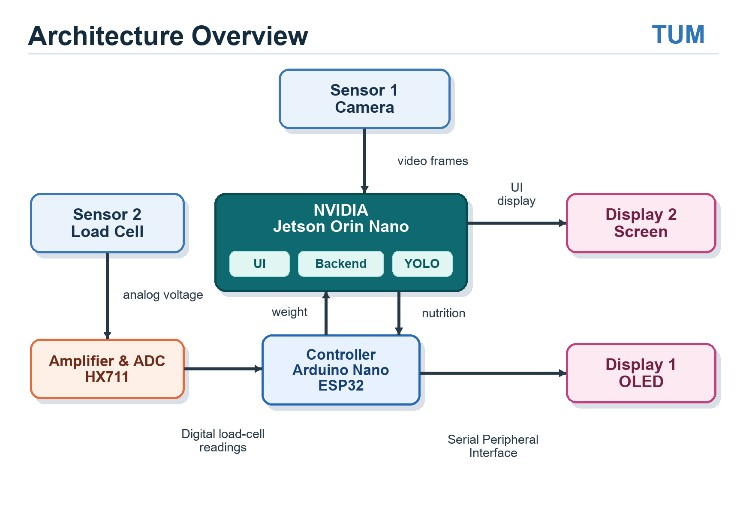
\includegraphics[width=0.7\textwidth]{system_architecture.jpg}
  \caption{System architecture of the Smart Calorie Plate, showing the camera and load-cell sensing paths, Jetson-based inference stack, Arduino Nano ESP32 controller, and OLED/screen feedback channels.}
  \label{fig:architecture}
\end{figure}

The two computing layers exchange only the values required for the nutrition loop. The controller sends weight measurements to the Jetson, while the Jetson returns calculated nutrition results for local display. A screen presents the main user interface from the Jetson, and the OLED provides lightweight peripheral feedback through the controller. This architecture supports real-time, offline meal analysis with minimal user input.

% =====================================================================
\section{Related Work}
% =====================================================================

Automatic dietary assessment has been studied from several technical directions, including image-based food recognition, portion-size estimation, and sensor-assisted nutrition tracking. Traditional calorie-tracking applications usually require users to manually search for food items, estimate portion sizes, and enter meal information. Although this method is simple to implement, it is time-consuming and often inaccurate because users may underestimate food weight or forget to record meals consistently.

Recent computer-vision-based approaches reduce this manual effort by recognizing food items from images. Deep learning models such as Faster R-CNN and YOLO have been widely used for object detection tasks, while segmentation models can provide more precise food boundaries. However, image-only systems still face an important limitation: they can identify what food is present, but they cannot reliably determine the actual mass of each food item. Since calorie calculation depends heavily on portion size, visual estimation alone may lead to large nutritional errors.

Other systems use electronic scales or smart kitchen devices to measure food weight accurately. These devices provide reliable mass measurements but usually cannot automatically identify the food type. As a result, users still need to manually input food names or select items from a database.

The Smart Calorie Plate combines these two directions. It uses a camera-based YOLOv11 segmentation model to recognize food categories and a load-cell-based weighing platform to measure food mass. By integrating visual recognition, weight measurement, local nutrition computation, and a desktop user interface on an edge-computing platform, the system reduces manual input while improving the reliability of calorie estimation.

% =====================================================================
\section{Deployment Platform: NVIDIA Jetson Orin Nano}
% =====================================================================

\subsection{Rationale for Edge Computing}

To satisfy the real-time and offline operation requirements of the smart calorie-tracking device, we adopted an edge-computing architecture rather than relying on cloud-based inference. The NVIDIA Jetson Orin Nano Developer Kit~\cite{jetson} serves as the primary single-board computer and hosts the complete application stack.

Compared with cloud-based processing, on-device inference provides three key advantages for this application:

\begin{itemize}
  \item \textbf{Low latency:} The system delivers nutrition results within two seconds of image capture, regardless of network conditions.
  \item \textbf{Data privacy:} All images are processed locally and never leave the device.
  \item \textbf{Operational autonomy:} The system remains fully functional without an internet connection.
\end{itemize}

\subsection{Hardware Configuration}

The NVIDIA Jetson Orin Nano used in this project provides the hardware specifications summarized in Table~\ref{tab:jetson}, all of which are relevant to the application workload.

\begin{table}[H]
  \centering
  \caption{Hardware configuration of the NVIDIA Jetson Orin Nano Developer Kit.}
  \label{tab:jetson}
  \begin{tabular}{ll}
    \toprule
    \textbf{Component} & \textbf{Specification} \\
    \midrule
    GPU              & 1024-core NVIDIA Ampere GPU with 32 Tensor Cores \\
    CPU              & 6-core Arm Cortex-A78AE v8.2 (64-bit) \\
    Memory           & 8\,GB 128-bit LPDDR5, shared between CPU and GPU \\
    AI performance   & Up to 40 TOPS (INT8) \\
    Storage          & microSD card (system and application storage) \\
    Camera input     & USB camera via \texttt{/dev/video0} (V4L2) \\
    Serial interface & USB serial \texttt{/dev/ttyACM0} (Arduino link) \\
    \bottomrule
  \end{tabular}
\end{table}

\subsection{Software Architecture}

On the Jetson, the application runs as a FastAPI backend process---orchestrated by \texttt{run\_app.py}---together with two companion scripts that bridge the camera and the Arduino to that backend. The backend process comprises three core subsystems:

\begin{enumerate}
  \item \textbf{YOLOv11 inference engine.} The trained model is loaded once at application startup through a thread-safe singleton and subsequently serves inference requests from the backend.
  \item \textbf{FastAPI backend with Uvicorn ASGI server.} The backend~\cite{fastapi} exposes a REST API for food detection and image analysis (\texttt{/meal/*}), food and nutrition data (\texttt{/foods}), and user profiles, meal logging, daily summaries, and recommendations (\texttt{/api/*}). The same server also serves the statically exported frontend from the root path, so the interface and the API share one origin.
  \item \textbf{SQLite database.} The local database stores nutritional information for 18 food categories and maintains the user's meal history.
\end{enumerate}

Two companion scripts handle the hardware I/O on the Jetson and communicate with the backend over its REST API rather than living inside the backend process:

\begin{enumerate}
  \setcounter{enumi}{3}
  \item \textbf{Camera capture.} A capture script reads frames from \texttt{/dev/video0} using OpenCV~\cite{opencv} and submits them to the backend's \texttt{/meal/detect} and \texttt{/meal/analyze-image} endpoints for recognition and nutritional analysis.
  \item \textbf{Arduino serial bridge.} A serial script continuously reads the compartment-weight messages (\texttt{DATA,w1,w2,w3,total}) from \texttt{/dev/ttyACM0} at 9{,}600 baud, and after nutritional values have been computed, transmits the results back to the Arduino (\texttt{NUTRI,kcal,protein,carbs,fat}) for presentation on the OLED display.
\end{enumerate}

The Next.js frontend is statically exported as HTML and JavaScript and served directly by the FastAPI application. This arrangement avoids cross-origin communication issues and simplifies deployment. A PyWebView desktop window renders the interface using GTK/WebKit, providing a native, kiosk-style user experience without requiring users to interact with a conventional web browser.

% =====================================================================
\section{Computer Vision Model: YOLOv11 Segmentation}
% =====================================================================

\subsection{Model Selection}

Following preliminary comparisons among YOLOv8, YOLOv11, and Faster R-CNN, we selected \textbf{YOLOv11n-seg}, the nano variant equipped with a segmentation head~\cite{ultralytics}. The model was chosen for three primary reasons.

\begin{enumerate}
  \item \textbf{Speed--accuracy balance.} In our initial evaluations, YOLOv11 achieved an approximately one- to two-percentage-point improvement in mAP@0.5 over YOLOv8 at a comparable parameter count. At the same time, it retained the computational efficiency of a single-stage detector and was capable of real-time inference on the Jetson platform.
  \item \textbf{Segmentation capability.} In addition to bounding boxes, the \texttt{-seg} variant generates pixel-level polygon masks. Although the current pipeline uses only predicted class labels and confidence scores, retaining segmentation output enables future extensions, such as estimating the visible surface area or approximate volume of individual food items, without requiring the model to be retrained.
  \item \textbf{Deployment maturity.} Ultralytics provides a unified workflow for exporting models from PyTorch to formats such as ONNX and TensorRT~\cite{ultralytics}. This streamlined export process substantially reduces the complexity of deploying the model on the Jetson platform.
\end{enumerate}

The nano variant was selected instead of the small or medium variants because its approximately 3.2 million parameters fit comfortably within the Jetson's 8\,GB of shared memory while leaving sufficient resources for the backend, database, user interface, and other device services. In addition, the larger variants did not produce a measurable improvement in accuracy for the project's relatively limited 18-class recognition task.

\subsection{Model Configuration}

The full training configuration is listed in Table~\ref{tab:training}.

\begin{table}[H]
  \centering
  \caption{YOLOv11n-seg training configuration.}
  \label{tab:training}
  \begin{tabular}{ll}
    \toprule
    \textbf{Parameter} & \textbf{Value} \\
    \midrule
    Base model        & \texttt{yolo11n-seg.pt} (COCO pre-trained) \\
    Input resolution  & $640 \times 640$ \\
    Epochs            & 100 \\
    Batch size        & 16 \\
    Optimizer         & SGD (Ultralytics default schedule) \\
    Data augmentation & Mosaic, HSV shift, random flip (defaults) \\
    Training hardware & Google Colab, NVIDIA T4 GPU \\
    Export format     & PyTorch \texttt{.pt} (FP32) \\
    \bottomrule
  \end{tabular}
\end{table}

\subsection{Class Alignment with Nutrition Database}

A subtle but important architectural decision was to align the model's class indices with the primary keys used in the nutrition database.

During dataset annotation, the food categories were assigned indices in strict alphabetical order, for example, banana${}=0$, beef${}=1$, and tomato${}=17$. The database seed script inserts the corresponding food records into SQLite in the same order, ensuring that each database food ID directly matches its YOLO class index.

This one-to-one alignment eliminates the need for a runtime class-name-to-database-ID mapping. As a result, the inference-to-nutrition pipeline can retrieve the corresponding nutritional record directly using the predicted class index, reducing implementation complexity and minimizing the possibility of mapping errors.

\subsection{Deployment Pipeline}

Training was performed off-device on Google Colab (T4 GPU) using the Ultralytics CLI~\cite{ultralytics}:

\begin{lstlisting}[language=bash]
yolo segment train model=yolo11n-seg.pt data=data.yaml \
    epochs=100 imgsz=640 batch=16
\end{lstlisting}

The resulting \texttt{best.pt} was transferred to the Jetson at \texttt{\textasciitilde/smart-calorie-plate/model/best.pt}. At Jetson startup, the model is instantiated once inside a thread-safe singleton:

\begin{lstlisting}[language=Python]
_model: YOLO | None = None
_lock = Lock()

def get_model():
    global _model
    if _model is None:
        with _lock:
            if _model is None:
                _model = YOLO(str(MODEL_PATH))
    return _model
\end{lstlisting}

\subsection{Model Performance}

Results measured on our held-out test set are summarized in Table~\ref{tab:performance}.

\begin{table}[H]
  \centering
  \caption{Overall model performance on the held-out deployment test set.}
  \label{tab:performance}
  \begin{tabular}{lc}
    \toprule
    \textbf{Metric} & \textbf{Value} \\
    \midrule
    mAP@0.5 (box)                  & 0.752 \\
    mAP@0.5:0.95 (box)             & 0.545 \\
    mAP@0.5 (mask)                 & 0.748 \\
    mAP@0.5:0.95 (mask)            & 0.531 \\
    Precision                      & 0.771 \\
    Recall                         & 0.716 \\
    Inference speed (Jetson, FP32) & $\approx$12 FPS \\
    Model size (\texttt{.pt})      & 5.7\,MB \\
    \bottomrule
  \end{tabular}
\end{table}

An 18-class YOLOv11n model reaching mAP@0.5${}\approx 0.75$ on a real-deployment test set is a reasonable outcome for a nano-scale architecture trained on a mid-sized custom dataset. The gap between mAP@0.5 and mAP@0.5:0.95 ($\sim$0.21) reflects the well-known tendency of nano detectors to produce slightly loose bounding boxes and masks---a mask-quality issue rather than a classification failure, and one that does not degrade downstream nutrition calculation. Fine-tuning a larger backbone (e.g.\ YOLOv11s or YOLOv11m) is expected to close both gaps, at the cost of higher inference latency on the Jetson.

\subsection{Per-Class Performance}

Table~\ref{tab:perclass} lists the precision, recall, and per-class mAP@0.5 for each of the 18 classes. The best-performing class (broccoli) and the weakest class (pork) are highlighted in bold.

\begin{table}[H]
  \centering
  \caption{Per-class detection performance on the held-out test set.}
  \label{tab:perclass}
  \begin{tabular}{lccc}
    \toprule
    \textbf{Class} & \textbf{Precision} & \textbf{Recall} & \textbf{mAP@0.5} \\
    \midrule
    banana              & 0.88 & 0.85 & 0.86 \\
    beef                & 0.68 & 0.65 & 0.65 \\
    bread               & 0.72 & 0.70 & 0.71 \\
    \textbf{broccoli}   & \textbf{0.90} & \textbf{0.92} & \textbf{0.90} \\
    carrot              & 0.85 & 0.82 & 0.83 \\
    chicken             & 0.62 & 0.65 & 0.60 \\
    cucumber            & 0.80 & 0.78 & 0.79 \\
    egg                 & 0.68 & 0.62 & 0.63 \\
    fish                & 0.72 & 0.68 & 0.68 \\
    juice               & 0.85 & 0.80 & 0.82 \\
    lemon               & 0.86 & 0.85 & 0.85 \\
    noodles             & 0.72 & 0.68 & 0.68 \\
    \textbf{pork}       & \textbf{0.58} & \textbf{0.62} & \textbf{0.58} \\
    potato              & 0.68 & 0.65 & 0.65 \\
    rice                & 0.75 & 0.72 & 0.72 \\
    sausage             & 0.80 & 0.75 & 0.76 \\
    strawberry          & 0.83 & 0.80 & 0.81 \\
    tomato              & 0.78 & 0.80 & 0.78 \\
    \bottomrule
  \end{tabular}
\end{table}

\subsection{Discussion}

Three patterns emerge from the per-class results. First, visually distinctive foods perform best: broccoli, banana, lemon, and carrot achieve the highest scores because their shapes and colors are easily distinguishable.

Second, meat classes perform weakest. Pork, chicken, beef, and fish share similar colors and textures after cooking, making them difficult to separate using RGB images alone. Future improvements could include collecting more diverse training samples or adding spectroscopic sensing.

Third, starches such as bread, potato, rice, and noodles, as well as strawberry and tomato, form smaller confusion groups due to their similar appearance. These errors have limited impact on calorie estimation because foods within each group have relatively similar nutritional profiles.

Overall, all 18 classes achieve an mAP@0.5 above 0.58. Most errors occur between visually similar foods, indicating that targeted data collection for these class pairs would provide the greatest improvement.

% =====================================================================
\section{Dataset Construction and Preparation}
% =====================================================================

\subsection{Data Source Strategy}

Assembling a training set that is both large enough for reliable convergence and specific enough to our real-world deployment posed the central data challenge. We adopted a three-source strategy to balance quantity, quality, and domain match:

\begin{enumerate}
  \item \textbf{Public dataset (FoodSeg103).} A subset of FoodSeg103 provided a strong initial base of professionally annotated food images. We filtered its 103 categories down to the 18 items relevant to our nutrition database, discarding non-matching classes. Representative samples are shown in Figure~\ref{fig:datasetsamples}.
  \item \textbf{Web-scraped images.} For under-represented classes (e.g.\ juice, strawberry), we augmented the set with search engine imagery. All scraped images were manually reviewed to remove logos, watermarks, and low-quality samples.
  \item \textbf{In-house captured images.} To close the domain gap between public data (typically shot at restaurant angles under warm lighting) and our target scenario (top-down view of a 3-compartment tray under LED illumination), we captured a targeted set of images using the actual hardware setup (Figure~\ref{fig:inhouse}).
\end{enumerate}

\begin{figure}[H]
  \centering
  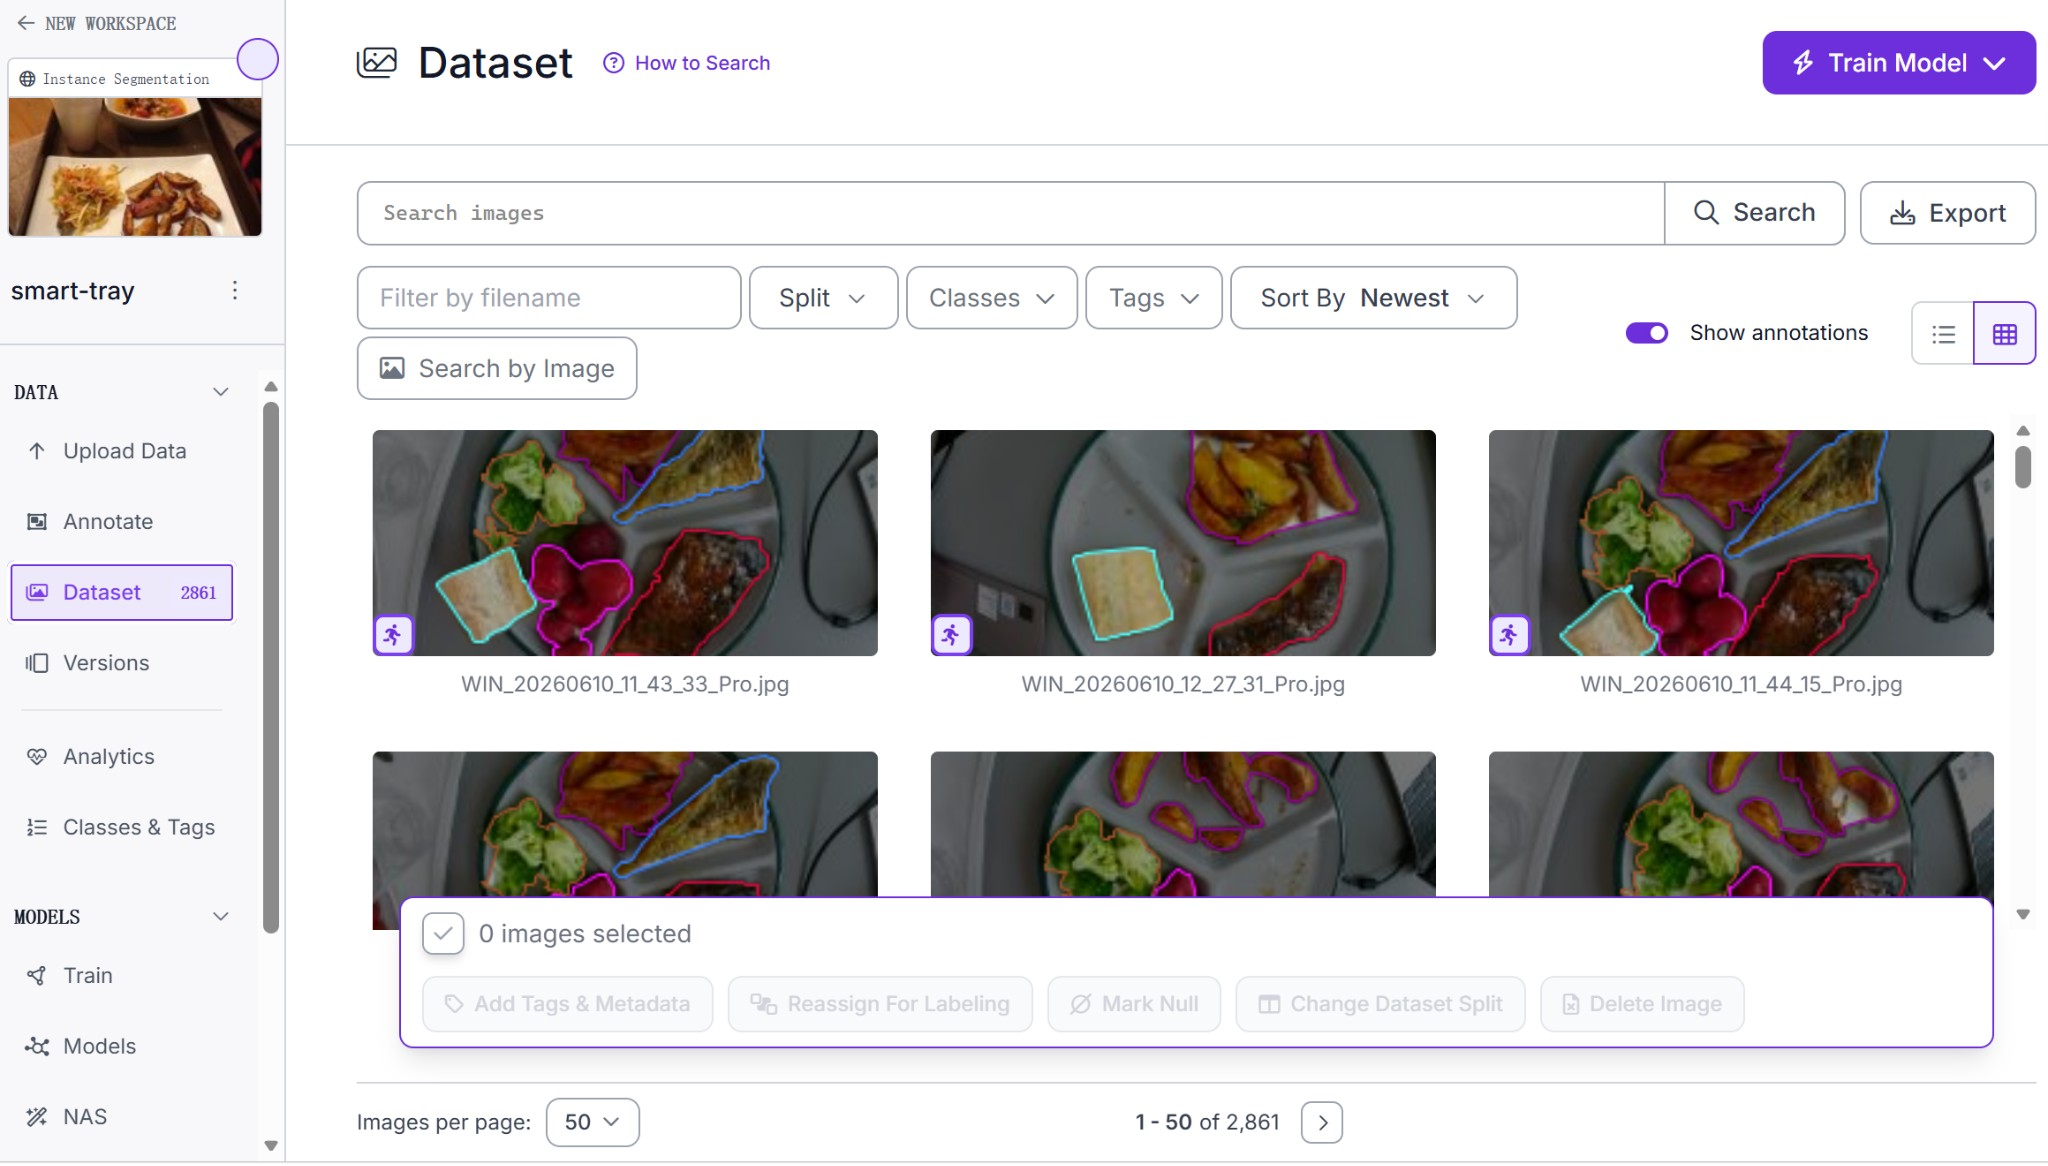
\includegraphics[width=0.85\textwidth]{dataset_samples.jpg}
  \caption{Representative annotated samples drawn from the filtered FoodSeg103 subset and web-scraped sources.}
  \label{fig:datasetsamples}
\end{figure}

\subsection{Annotation Pipeline}

All annotations were performed on the Roboflow platform~\cite{roboflow}, which provides a collaborative web interface and native YOLOv11 segmentation export. We chose polygon segmentation over bounding boxes for two reasons: (i) it produces tighter object contours that improve model accuracy in the crowded scenes typical of a multi-food plate; and (ii) the polygon vertices are usable for future per-food area or portion-size estimation.

Class IDs were assigned in strict alphabetical order ($0={}$banana, $1={}$beef, \ldots, $17={}$tomato). This convention, applied consistently across all three data sources, guarantees direct alignment with the nutrition database's food IDs.

\subsection{Train / Validation / Test Split}

The dataset of 2{,}861 annotated images was partitioned into 2{,}232 training, 420 validation, and 209 test images (approximately 78\,/\,15\,/\,7\%). The validation set was consulted after every training epoch to select the best model checkpoint. The test set remained untouched throughout training and was used exclusively for the final metrics.

Unlike the training and validation subsets, which draw from the combined public, web-scraped, and in-house image pool, the test subset was deliberately composed of photographs taken with the actual deployed hardware. A fixed acrylic test tray was photographed under multiple lighting conditions using the same top-down camera setup used in the final system, rather than relying on additional public or web-sourced images. This ensured that the reported test performance reflects real deployment conditions rather than the more visually consistent distribution of the training data.

\begin{figure}[H]
  \centering
  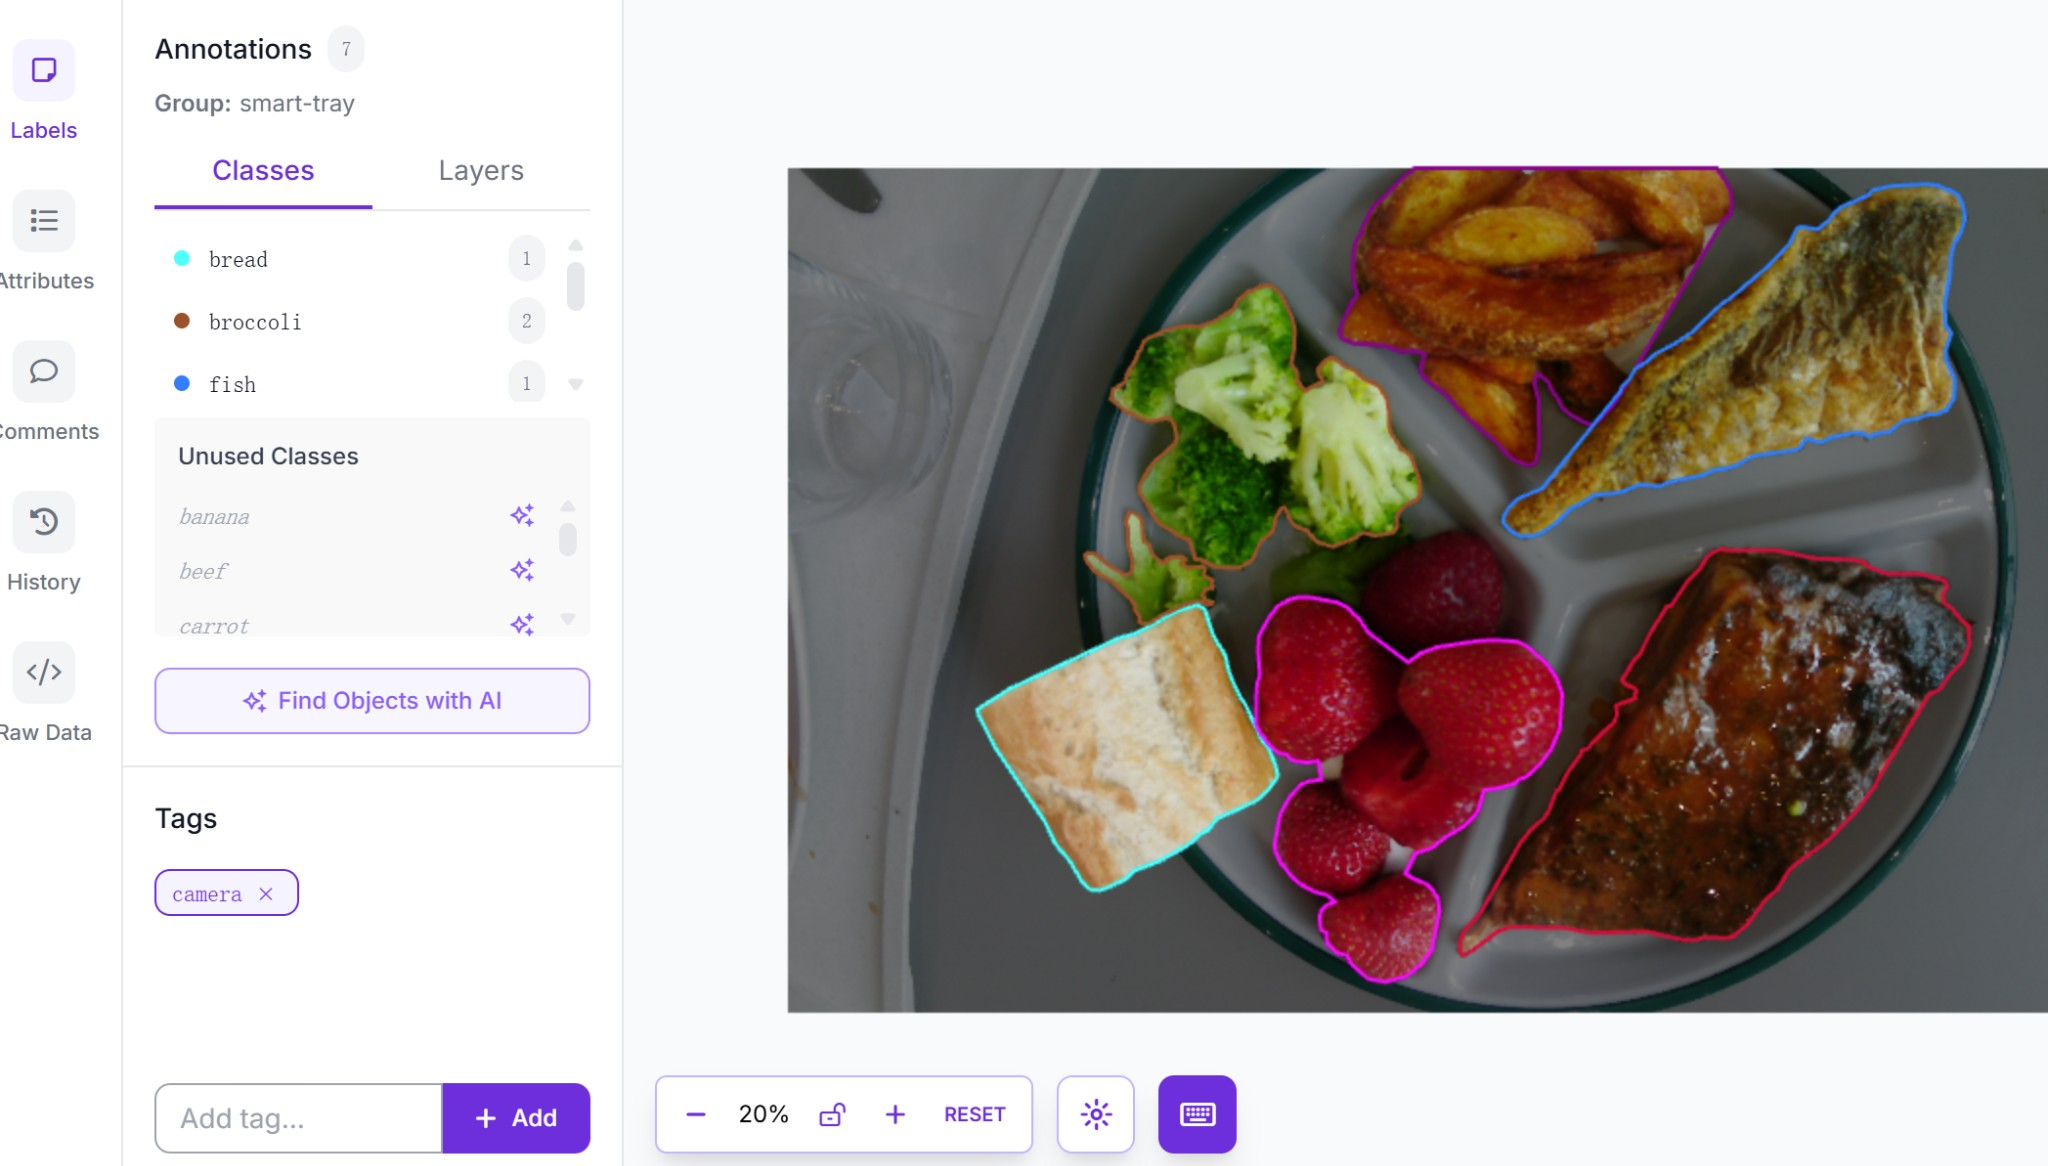
\includegraphics[width=0.85\textwidth]{inhouse_images.jpg}
  \caption{In-house captured training images: top-down views of the three-compartment tray under the deployed camera and lighting setup.}
  \label{fig:inhouse}
\end{figure}

\subsection{Dataset Challenges}

Beyond assembling a sufficiently large and well-annotated dataset, an important part of the preparation process involved identifying which food categories were harder for the model to recognize and required targeted improvement. After each training iteration, per-class validation performance was cross-referenced with the class distribution recorded in Roboflow~\cite{roboflow} to decide where additional data collection was needed. This process revealed a clear class imbalance across the 18 categories---for example, broccoli was represented by over 2{,}100 annotated instances, while banana had only 154. The recorded per-class instance distribution is shown in Figure~\ref{fig:distribution}, and the resulting balance analysis in Figure~\ref{fig:balance}.

Categories with limited representation, irregular shape, or visual similarity to the tray or to other foods consistently produced lower detection confidence during testing. Based on these findings, we prioritized targeted image collection and re-annotation for under-represented or low-confidence classes in subsequent dataset iterations, rather than expanding the entire dataset uniformly. This class-by-class refinement approach improved recognition reliability without disproportionately increasing annotation workload. The fixed test tray used for deployment-condition evaluation is shown in Figure~\ref{fig:testtray}.

\subsection{Final Dataset Overview}

The final dataset comprises 2{,}861 annotated images across 18 categories, expanded to approximately 7{,}345 training examples after augmentation (mosaic + HSV shift + random flip). Validation and test subsets use 420 and 209 original images respectively. The dataset combines public, web-sourced, and in-house captured images to bridge the gap between generic food-recognition benchmarks and our top-down, tray-based deployment scenario. To ensure evaluation results were representative of real operating conditions, the held-out test set consisted exclusively of photographs captured with the deployed hardware---a fixed test tray photographed under varying lighting using the actual camera setup. Combined with the iterative, class-level refinement process described above, this dataset strategy provided a deployment-relevant foundation for training the YOLOv11 segmentation model used in the final system.

\begin{figure}[H]
  \centering
  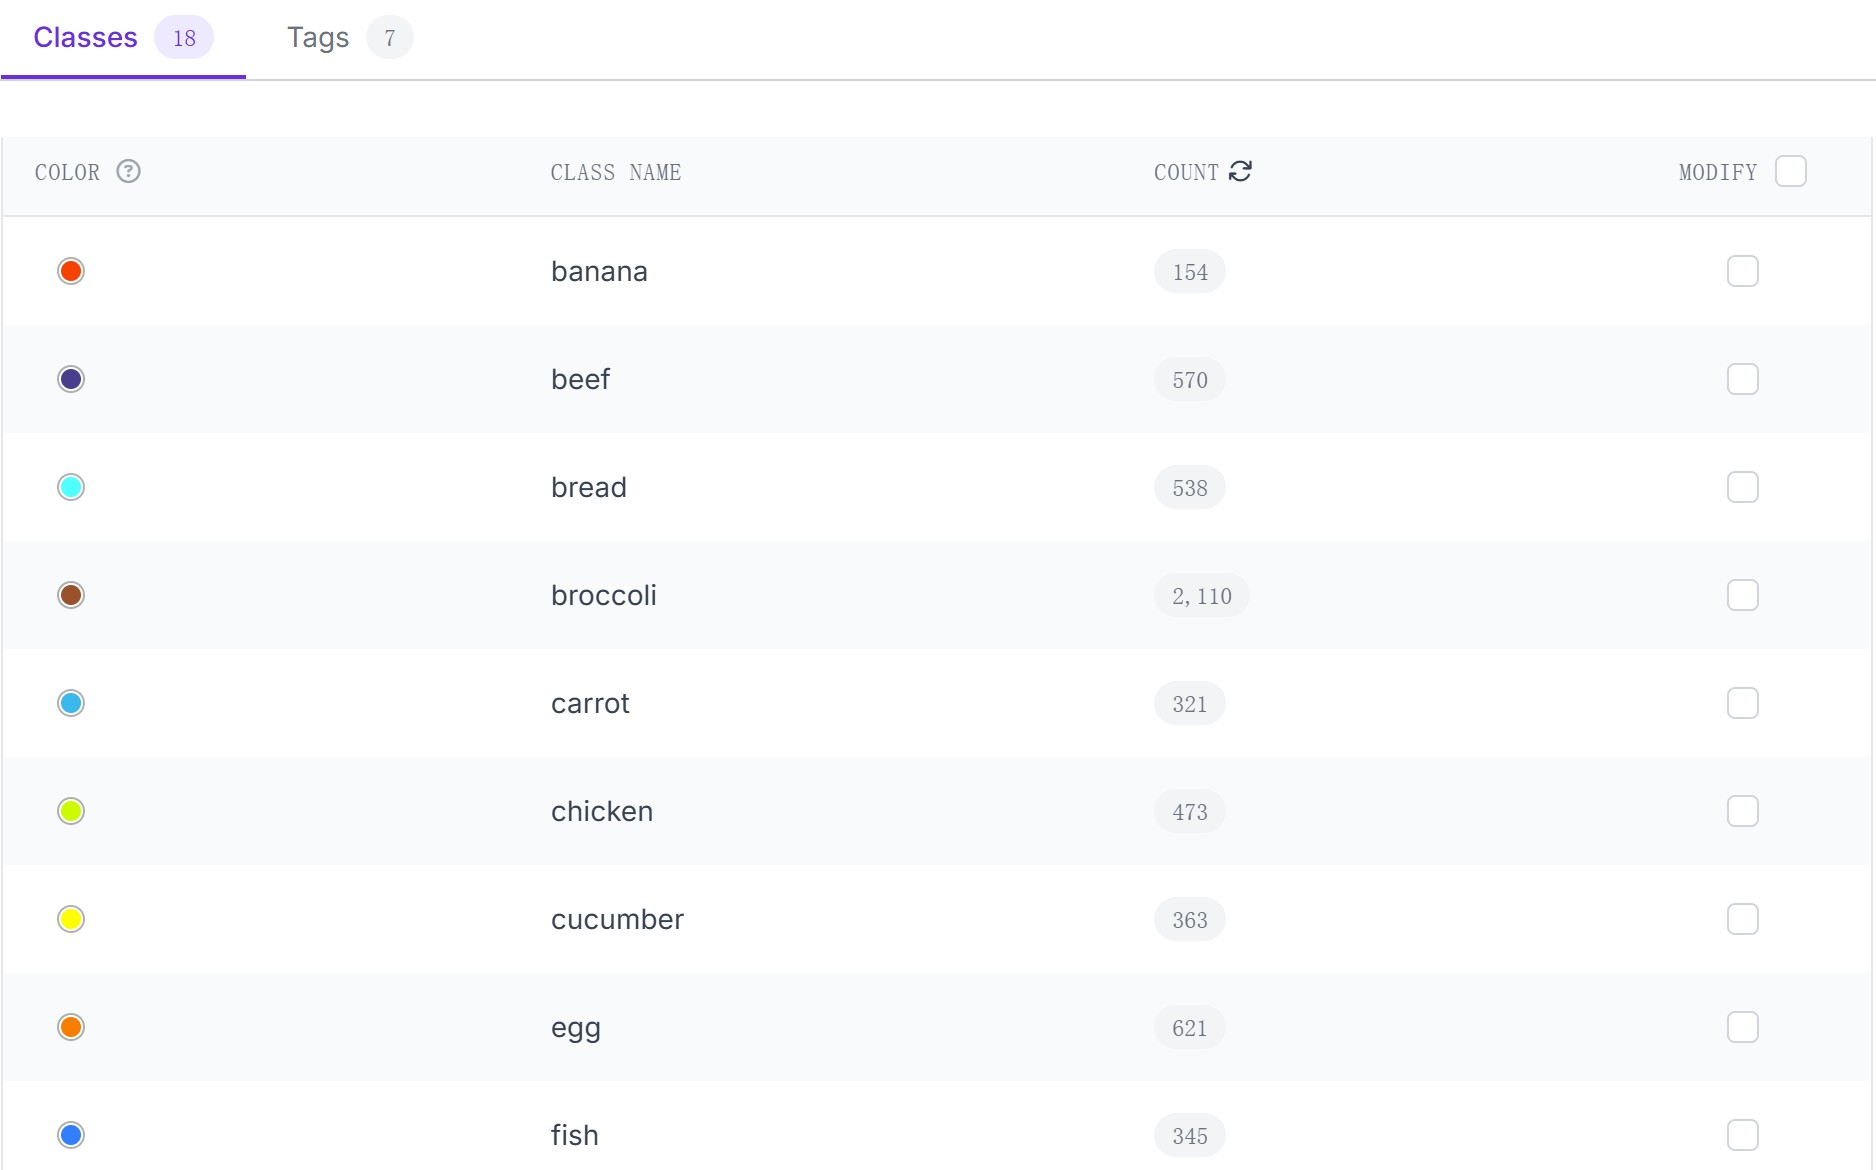
\includegraphics[width=0.85\textwidth]{class_distribution.jpg}
  \caption{Per-class annotated instance counts recorded in Roboflow, revealing a pronounced class imbalance across the 18 food categories.}
  \label{fig:distribution}
\end{figure}

\begin{figure}[H]
  \centering
  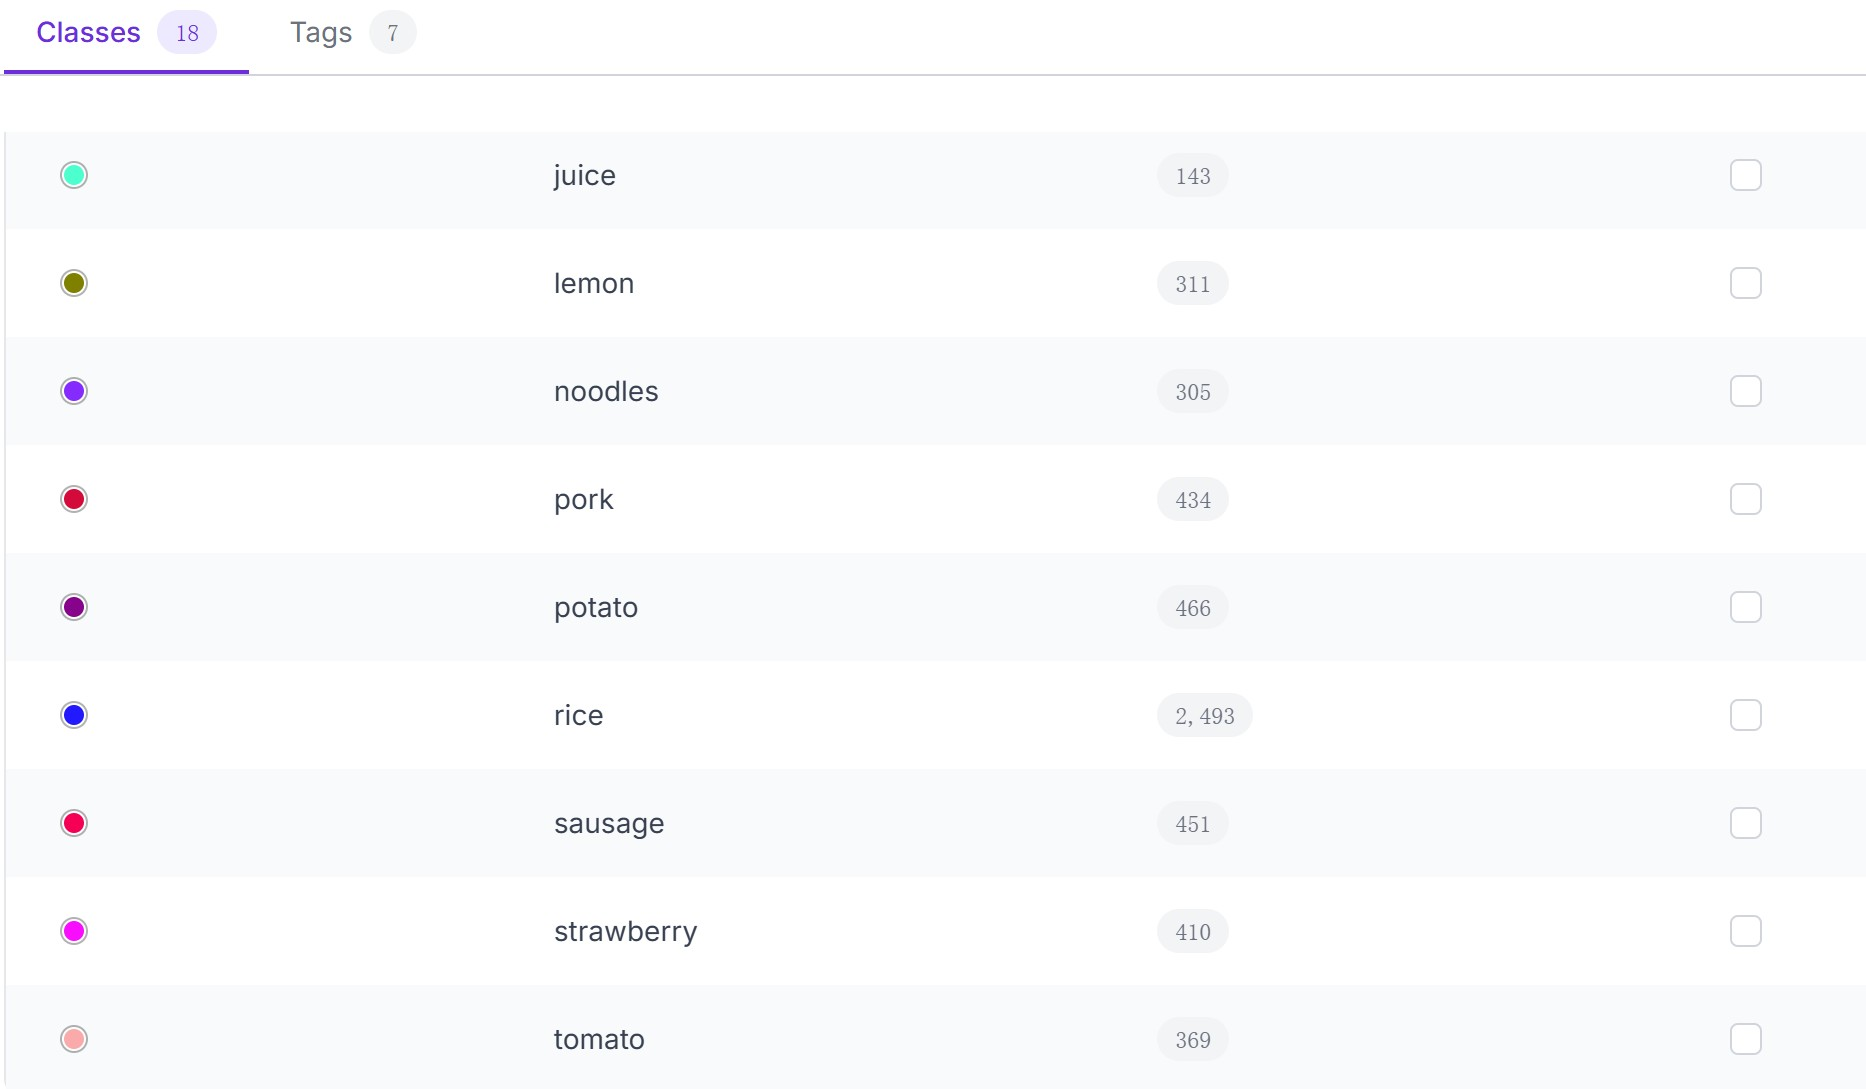
\includegraphics[width=0.85\textwidth]{class_balance.jpg}
  \caption{Class balance analysis used to prioritize targeted data collection for under-represented categories.}
  \label{fig:balance}
\end{figure}

\begin{figure}[H]
  \centering
  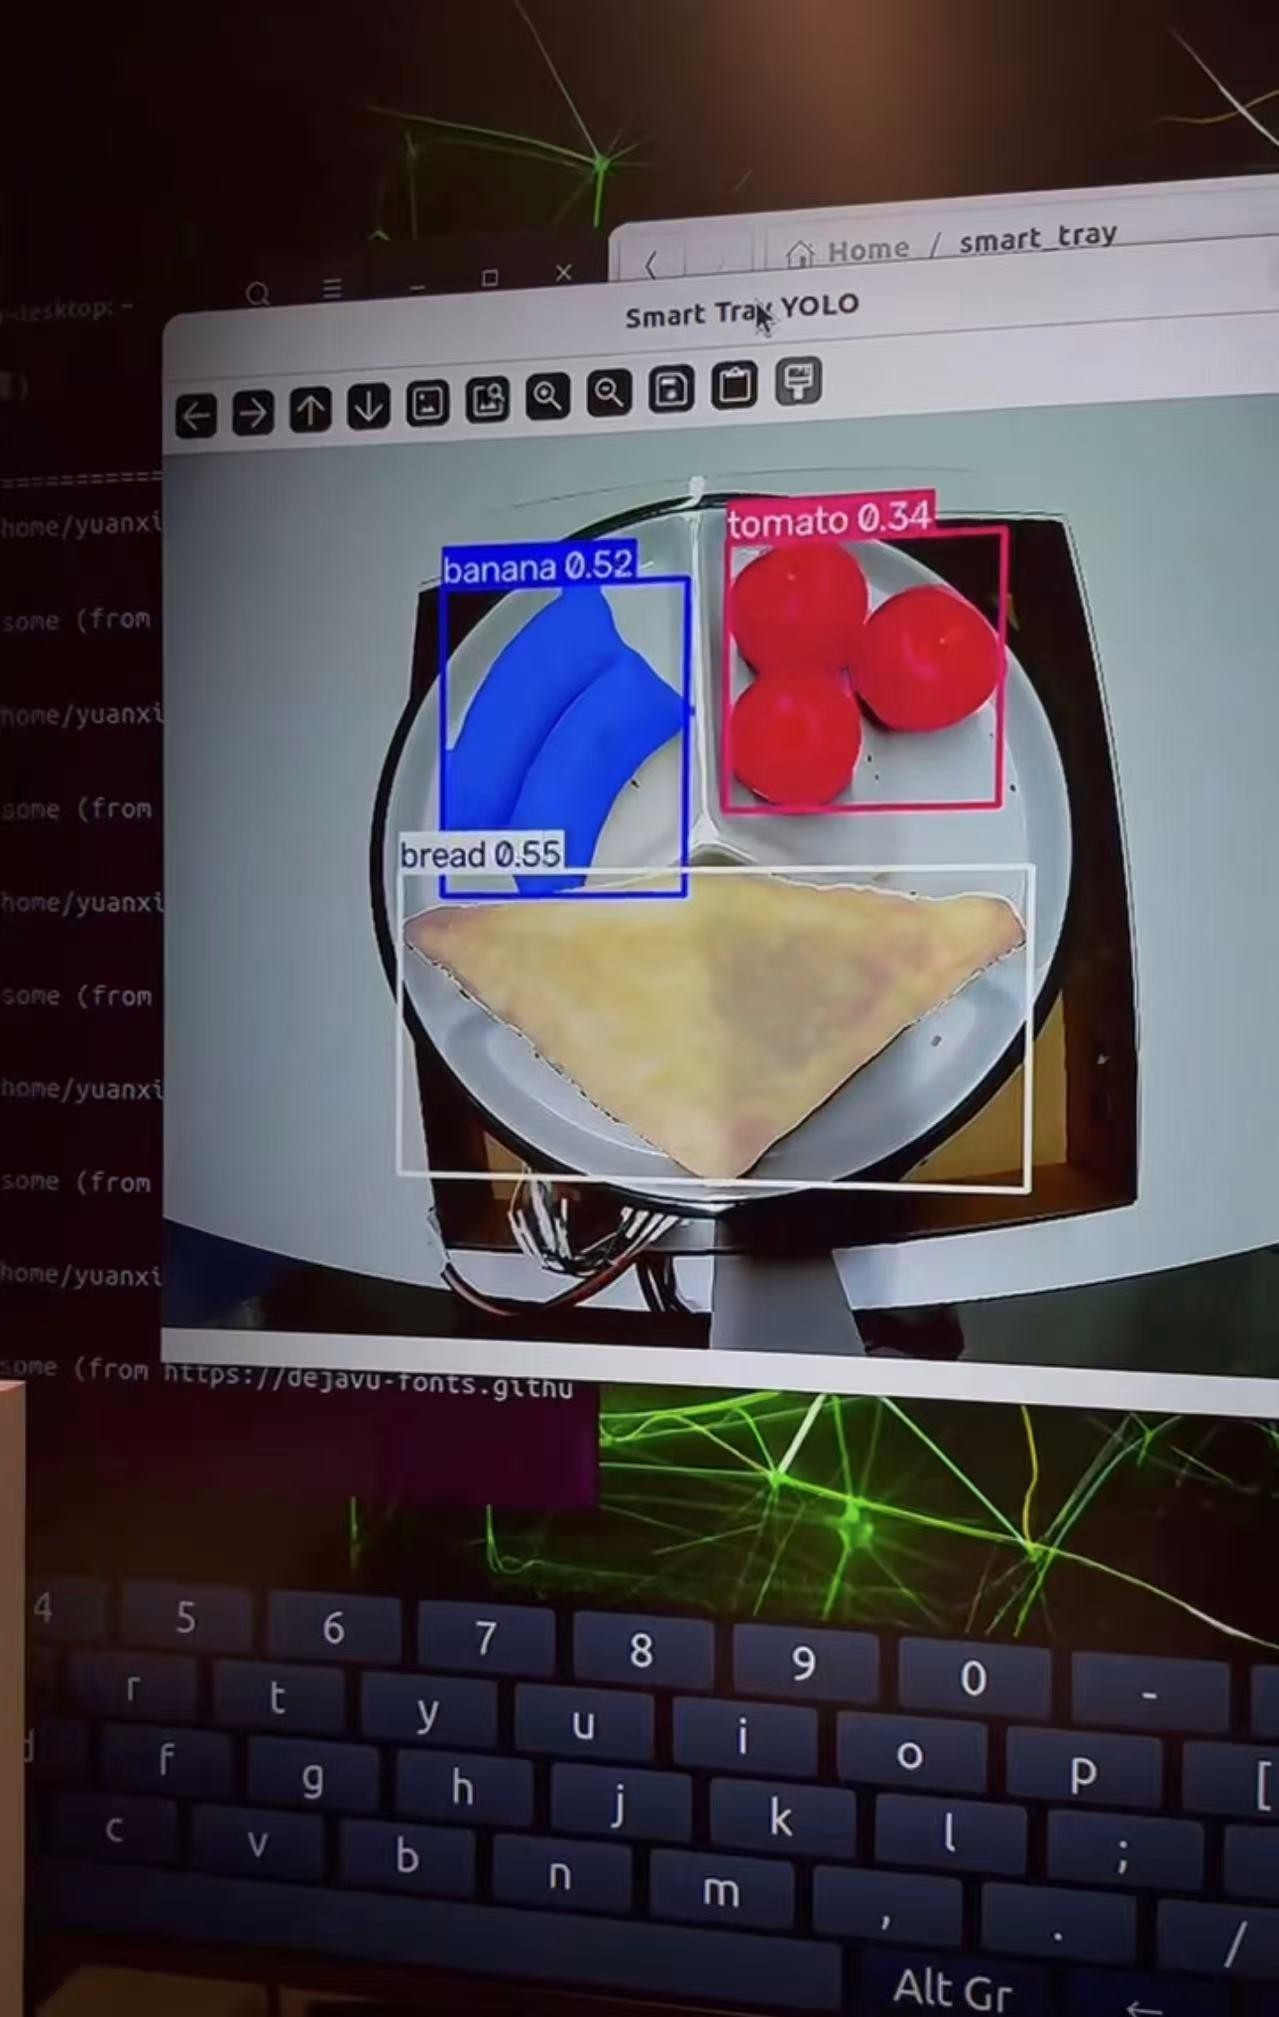
\includegraphics[width=0.45\textwidth]{test_tray.jpg}
  \caption{Fixed acrylic test tray photographed with the deployed top-down camera setup, used exclusively for the held-out test set.}
  \label{fig:testtray}
\end{figure}

% =====================================================================
\section{Mechanical Structure Design}
% =====================================================================

The mechanical structure of the smart calorie plate was designed to integrate the camera system, weighing platform, load cells, and electronic enclosure into a stable and functional device. The design process focused on ensuring accurate food recognition, reliable weight measurement, and ease of assembly.

\subsection{Camera Support Structure}

To support food recognition, a dedicated camera stand was designed using Tinkercad (Figure~\ref{fig:camerastand}). Since the camera is responsible for capturing images of the food container, it was important to position it directly above the weighing platform. Several placement options were considered, and a top-view configuration was selected because it allows the entire bowl to remain within the camera's field of view while reducing image distortion. The height of the camera stand was determined based on the size of the weighing platform and the desired image coverage area. To improve structural stability, an interlocking tab-and-slot design was incorporated into the support structure. The final camera stand was manufactured using a 3D printer and mounted above the platform.

\begin{figure}[H]
  \centering
  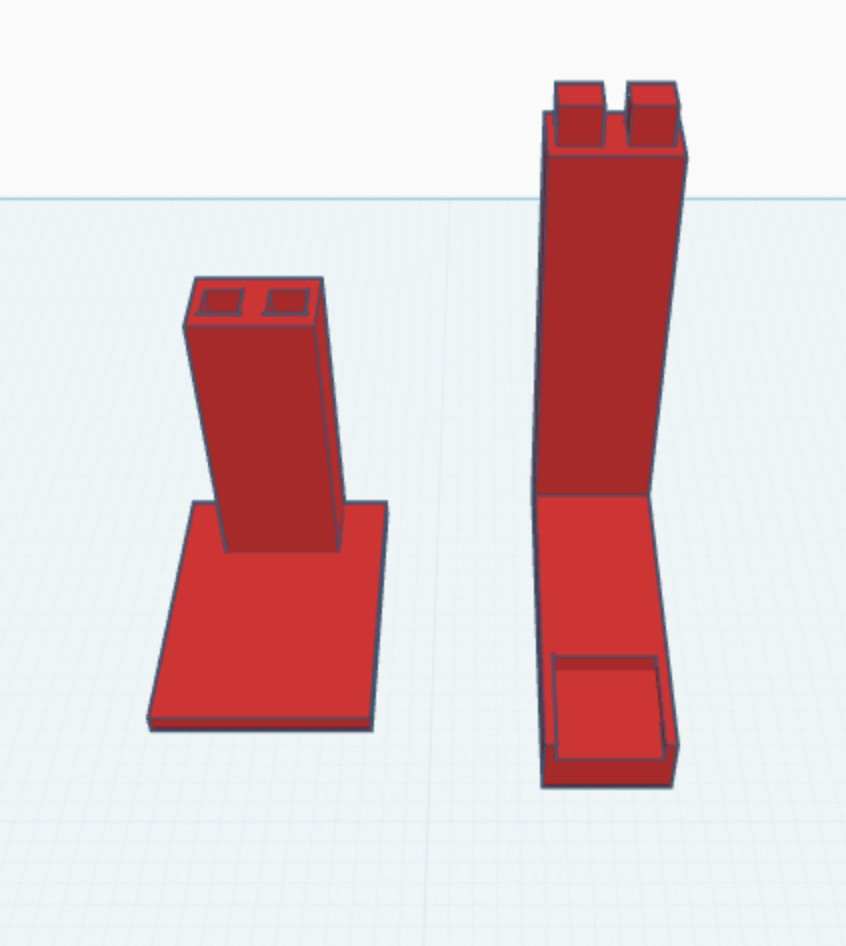
\includegraphics[width=0.4\textwidth]{camera_stand.jpg}
  \caption{CAD model of the 3D-printed camera support structure designed in Tinkercad, featuring an interlocking tab-and-slot assembly.}
  \label{fig:camerastand}
\end{figure}

\subsection{Enclosure Design}

A wooden enclosure was also designed to house the electronic components of the system. The enclosure serves as the base structure and provides protection for the internal hardware, including the controller board, sensors, and wiring. The enclosure panels were designed for laser cutting and assembled using an interlocking tab-and-slot structure. This approach simplifies assembly while improving rigidity. In addition, ventilation openings were included to improve heat dissipation, and cable-routing openings were added to simplify wiring and maintenance.

\subsection{Weighing Platform and Load Cell Layout}

The weighing platform was constructed using a circular acrylic plate with a diameter of 250\,mm. A circular geometry was selected because it provides a natural and convenient placement area for bowls and food containers. To achieve stable weight measurement, four load cells were positioned symmetrically around the center of the platform. The placement locations were determined by first locating the center of the acrylic plate and then arranging the sensors in a balanced square-like configuration around that center. This design helps distribute the applied load among all sensors and improves measurement stability.

Before fabrication, the dimensions of the load cells were measured using a vernier caliper to determine the required mounting locations and screw sizes. Based on these measurements, mounting holes were drilled into the acrylic platform. M4 screws were selected for fastening because they provided sufficient mechanical strength and compatibility with the load cells. After drilling and assembly, the sensors were securely attached to the platform to form the weighing subsystem.

\subsection{Final Assembly}

The final mechanical structure combines 3D-printed components, laser-cut wooden parts, and a custom acrylic weighing platform. This design provides a stable foundation for image acquisition and weight measurement while allowing future modifications and upgrades to the system.

% =====================================================================
\section{Weight Measurement Module}
% =====================================================================

\subsection{Hardware Design}

The weighing module is responsible for measuring the food weight in the three compartments of the smart plate. It provides the weight data required by the subsequent food-recognition and nutritional-analysis modules.

The hardware consists of four load cells, four HX711 amplifier and analog-to-digital converter modules, one Arduino Nano ESP32, and one OLED display. The electrical signal generated by a load cell is only a few millivolts and therefore cannot be measured directly by the microcontroller. Each load cell is consequently connected to an individual HX711 module, which amplifies the signal and converts it into a high-resolution digital value.

All components are connected using jumper wires and breadboards instead of a custom printed circuit board. This prototype-oriented configuration simplified hardware assembly, troubleshooting, and the replacement of individual sensors during development.

The Arduino Nano ESP32 acts as the controller of the weighing module. It reads the four HX711 modules, removes the zero-load offsets, calculates the three compartment weights, filters unstable values, displays the results on the OLED, and transmits the processed measurements through serial communication.

During startup, the system displays an instruction to keep the plate empty and waits five seconds before automatically performing the tare operation. A manual tare operation is also available. When the Arduino receives the character \texttt{t} or \texttt{T} through the serial interface, it displays the same five-second waiting message and then records new zero-load reference values.

\subsection{Calibration and Weight Estimation}

Unlike a conventional electronic scale, the smart plate contains three food compartments mounted on one shared acrylic platform. Therefore, a load applied to one compartment affects several load cells simultaneously. A direct one-to-one mapping between one load cell and one compartment is consequently not possible.

To account for this mechanical coupling, a multivariable linear calibration model was developed. A 40\,g reference weight was placed in seven loading configurations:

\begin{enumerate}
  \item Compartment 1
  \item Compartment 2
  \item Compartment 3
  \item Compartments 1 and 2
  \item Compartments 1 and 3
  \item Compartments 2 and 3
  \item Compartments 1, 2, and 3
\end{enumerate}

For combined configurations, a separate 40\,g reference weight was placed in each selected compartment. For example, the configuration involving Compartments 1 and 2 contained 40\,g in each compartment and therefore represented a total load of 80\,g.

For every configuration, the outputs of all four load cells were recorded simultaneously. These measurements were used to derive the calibration coefficients for the three compartment-weight equations.

Before weight estimation, the zero-load value recorded during the tare operation is subtracted from each current sensor reading. The resulting tare-compensated deviations are calculated as
\begin{equation}
  d_i = r_i - z_i, \qquad i = 1, \ldots, 4,
  \label{eq:deviation}
\end{equation}
where $r_i$ is the current reading of load cell $i$ and $z_i$ is its zero-load reference.

The estimated weight of each compartment $j$ is then calculated from all four tare-compensated sensor deviations:
\begin{equation}
  w_j = b_j + a_{j1} d_1 + a_{j2} d_2 + a_{j3} d_3 + a_{j4} d_4, \qquad j = 1, 2, 3.
  \label{eq:weight}
\end{equation}

In the Arduino implementation, the three equations of Eq.~\eqref{eq:weight} are evaluated as follows:

\begin{lstlisting}[language=C]
w1Raw = C1_BIAS + C1_L1*d1 + C1_L2*d2 + C1_L3*d3 + C1_L4*d4;
w2Raw = C2_BIAS + C2_L1*d1 + C2_L2*d2 + C2_L3*d3 + C2_L4*d4;
w3Raw = C3_BIAS + C3_L1*d1 + C3_L2*d2 + C3_L3*d3 + C3_L4*d4;
\end{lstlisting}

Each compartment therefore has its own bias term and four calibration coefficients. However, all three equations use the same four sensor deviations as inputs.

The calibration coefficients are stored as constants in the Arduino firmware. Therefore, the calibration model does not need to be recalculated during normal operation. The microcontroller only performs the required multiplications and additions, which allows the three compartment weights to be estimated in real time with low computational cost.

\subsection{Signal Processing and Software Implementation}

During normal operation, the Arduino reads five consecutive samples from each HX711 module and calculates their average. Averaging reduces short-term fluctuations and random sensor noise. During the tare procedure, thirty samples are averaged to obtain more stable zero-load references.

Before applying the calibrated linear model, the system first performs a no-load check. The absolute values of the four tare-compensated sensor deviations are added together to obtain \texttt{sumAbsD}:

\begin{lstlisting}[language=C]
long sumAbsD = labs(d1) + labs(d2) + labs(d3) + labs(d4);
if (sumAbsD < NO_LOAD_SUM_THRESHOLD) {
    w1Raw = 0.0; w2Raw = 0.0; w3Raw = 0.0;
}
\end{lstlisting}

If the combined tare-compensated sensor deviation, represented by \texttt{sumAbsD}, is below the predefined no-load threshold of 2500, the plate is treated as empty and all three compartment weights are immediately set to zero. In this case, the linear estimation equations are not evaluated.

This no-load check is different from the dead-band filter. The no-load check evaluates the combined deviations of all four sensors before weight estimation, whereas the dead-band filter is applied separately to each calculated compartment weight afterwards.

After the linear weight estimation, the following post-processing steps are applied:

\begin{enumerate}
  \item Values with an absolute magnitude below 8\,g are treated as noise and set to zero.
  \item Negative values are set to zero.
  \item Valid measurements are rounded to the nearest gram.
\end{enumerate}

The corresponding function is shown below:

\begin{lstlisting}[language=C]
float cleanWeight(float w) {
    if (fabs(w) < COMP_DEADBAND_G) return 0.0;
    if (w < 0) return 0.0;
    return roundToStep(w, ROUND_STEP_G);
}
\end{lstlisting}

The three processed compartment values are then added to calculate the total food weight:

\begin{lstlisting}[language=C]
float w1 = cleanWeight(w1Raw);
float w2 = cleanWeight(w2Raw);
float w3 = cleanWeight(w3Raw);
float totalW = w1 + w2 + w3;
\end{lstlisting}

These processing stages reduce visible fluctuations and prevent small sensor deviations from being interpreted as actual food weight.

\subsection{OLED Display and System Integration}

Before nutritional information is received, the OLED displays the individual weights of the three compartments together with their total weight.

The Arduino also transmits the processed weight values to the Jetson through a comma-separated serial message in the following format:

\begin{lstlisting}
DATA,w1,w2,w3,total
\end{lstlisting}

The actual implementation transmits the weight values without decimal places:

\begin{lstlisting}[language=C]
Serial.print("DATA,");
Serial.print(w1, 0); Serial.print(",");
Serial.print(w2, 0); Serial.print(",");
Serial.print(w3, 0); Serial.print(",");
Serial.println(totalW, 0);
\end{lstlisting}

After food recognition and nutritional calculation, the Jetson sends the nutritional result back to the Arduino using the following message format:

\begin{lstlisting}
NUTRI,kcal,protein,carbs,fat
\end{lstlisting}

The Arduino first uses the \texttt{NUTRI} keyword to identify the message type and then parses the four numeric fields that follow: calories, protein, carbohydrates, and fat.

After the first valid \texttt{NUTRI} message is received, the OLED switches from weight mode to nutrition mode. The nutrition display presents the calculated calorie value as well as the amounts of protein, carbohydrates, and fat.

The nutrition display remains active instead of automatically returning to the weight display after a fixed period. It is updated whenever a new \texttt{NUTRI} message is received and returns to weight mode only when another tare operation is performed, either during the next startup or through the manual \texttt{t} or \texttt{T} command.

This bidirectional serial protocol connects the low-level sensing and weight-processing functions of the Arduino with the image-processing and nutritional-analysis functions of the Jetson.

% =====================================================================
\section{Software}
% =====================================================================

The backend is implemented in Python using FastAPI~\cite{fastapi}, which exposes the recognition, analysis, and logging functionality as a REST API. SQLModel serves as both the ORM layer and the schema definition for the underlying SQLite database, so each Python class doubles as a database table:

\begin{lstlisting}[language=Python]
class Food(SQLModel, table=True):
    id: int | None = Field(default=None, primary_key=True)
    name_en: str
    kcal_per_100g: float
\end{lstlisting}

Food recognition is powered by the Ultralytics framework~\cite{ultralytics} running a YOLOv11n-seg model, with OpenCV and NumPy~\cite{opencv} handling image decoding and preprocessing:

\begin{lstlisting}[language=Python]
from ultralytics import YOLO
import cv2, numpy as np
\end{lstlisting}

The frontend is a Next.js (React + TypeScript) single-page application styled with Tailwind CSS. It is exported as a static site and rendered inside a PyWebView desktop window, so no browser installation or separate frontend server is required at runtime.

\subsection{Food Recognition Pipeline}

Incoming image bytes---from a file upload or a live camera frame---are decoded with OpenCV and passed to the YOLO model. Because model loading takes several seconds, the model is instantiated lazily as a thread-safe singleton and reused across all requests:

\begin{lstlisting}[language=Python]
if _model is None:
    with _model_lock:
        _model = YOLO(str(MODEL_PATH))
\end{lstlisting}

The decisive design contract of the pipeline is the mapping between the vision model and the nutrition database: YOLO class indices are assigned alphabetically at training time, and the 18 seed foods are inserted with matching primary keys. A detection therefore resolves to a database row without any lookup table:

\begin{lstlisting}[language=Python]
food_id = int(cls_tensor.item())  # YOLO class index == Food.id
\end{lstlisting}

Each detection is returned with its confidence score, and the backend enriches it with the bilingual food names before sending it to the frontend for weight assignment.

\subsection{Nutrition Computation}

Personalized targets are derived in three stages. First, the basal metabolic rate (BMR) is computed with the Mifflin--St~Jeor equation~\cite{mifflin} from age, gender, height, and weight:
\begin{equation}
  \mathrm{BMR} = 10\,w + 6.25\,h - 5\,a + s, \qquad
  s =
  \begin{cases}
    +5   & \text{male},\\
    -161 & \text{female},
  \end{cases}
  \label{eq:bmr}
\end{equation}
where $w$ is the body weight in kg, $h$ is the height in cm, and $a$ is the age in years. The gender-specific offset $s$ follows the original Mifflin--St~Jeor formulation. The BMR is then scaled by an activity factor (1.2--1.725) into the total daily energy expenditure (TDEE), and finally adjusted by diet mode: $-400$\,kcal for fat loss, $+300$\,kcal for muscle gain, and no adjustment in maintenance mode. Equation~\eqref{eq:bmr} is implemented with an explicit gender branch, so all three diet modes inherit the correct male/female baseline:

\begin{lstlisting}[language=Python]
s = 5 if gender == "male" else -161
bmr = 10 * weight_kg + 6.25 * height_cm - 5 * age + s
tdee = bmr * activity_level
\end{lstlisting}

Macronutrients are allocated per kilogram of body weight (2.0\,g/kg protein in fat-loss and bulking modes, 1.8\,g/kg protein in maintenance mode, 0.9\,g/kg fat), and carbohydrates close the remaining calorie budget so that the three macros always sum to the calorie target:

\begin{lstlisting}[language=Python]
remaining_kcal = target_calories - (target_protein_g * 4
    + target_fat_g * 9)
target_carbs_g = max(0.0, remaining_kcal / 4.0)
\end{lstlisting}

For each meal, the sensor-reported weight scales the per-100\,g nutrient values of every detected food; totals are accumulated and compared against the remaining daily budget to generate rule-based advice and food suggestions ranked by the deficient macro.

\subsection{Desktop Deployment}

The application ships as a single desktop program. On launch, \texttt{run\_app.py} starts uvicorn on a background thread, polls the \texttt{/api/health} endpoint until the backend is ready, and only then opens a PyWebView window---preventing the user from ever seeing a half-initialized page.

\begin{lstlisting}[language=Python]
threading.Thread(target=_start_backend, daemon=True).start()
webview.create_window(title="Smart Plate", url=BASE_URL)
\end{lstlisting}

Crucially, FastAPI also serves the statically exported Next.js site, mounted at the root path after all API routes. Frontend and backend therefore share one origin and one port, which eliminates CORS configuration in production and avoids the classic packaged-app failure mode where pages opened via \texttt{file://} cannot load scripts or navigate:

\begin{lstlisting}[language=Python]
app.mount("/", StaticFiles(directory=str(FRONTEND_DIR), html=True))
\end{lstlisting}

As a resilience measure, the frontend degrades gracefully: if the backend is unreachable, nutrition targets are recomputed client-side with the same formulas, keeping the interface fully navigable offline.

% =====================================================================
\section{Limitations}
% =====================================================================

The current system still has several limitations. First, food recognition is limited to the categories included in the training dataset. Since the model was trained on 18 predefined food classes, foods outside this category set cannot be recognized reliably. If an unknown food is placed on the plate, the model may either fail to detect it or incorrectly classify it as one of the known categories.

Second, the system assumes a single-plate, top-down-view scenario under relatively controlled lighting conditions. The camera position, plate layout, and lighting environment are important for stable recognition. If the camera angle changes significantly, the plate is placed incorrectly, or the lighting becomes too dark or too reflective, the detection accuracy may decrease.

Third, mixed or overlapping foods can reduce detection confidence. When different foods are placed too close together, partially cover each other, or have similar colors and textures, the segmentation model may produce inaccurate masks or confused class predictions. This is especially challenging for visually similar foods such as meat or starch-based items.

Finally, calorie estimation relies mainly on the detected food category and the measured weight. The system does not analyze the exact recipe, cooking method, sauce, oil content, or ingredient composition of each food item. Therefore, the calculated calories should be understood as an estimation based on standard nutrition values rather than an exact nutritional measurement.

% =====================================================================
\section{Future Work}
% =====================================================================

Future work can address these limitations in several directions. First, the training dataset should be expanded to include more food categories, cooking styles, and real-world meal examples. Increasing the number and diversity of food classes would allow the system to recognize a wider range of meals and reduce incorrect classification of unknown foods.

Second, the hardware and vision pipeline can be improved to support more flexible deployment conditions. Future versions could include automatic lighting adjustment, image normalization, or a more robust camera calibration process. These improvements would make the system less dependent on a fixed top-down view and controlled lighting environment.

Third, the segmentation pipeline can be further developed to better handle mixed and overlapping foods. The system could use mask area, compartment location, confidence thresholds, and user confirmation to separate foods more accurately. Additional training images containing overlapping and mixed food arrangements would also help improve model robustness.

Finally, nutrition estimation can be improved by incorporating more detailed food information. Future versions could allow users to select cooking methods, add sauces or ingredients, and adjust recipe information manually. The system could also connect to a larger nutrition database so that calorie and macronutrient results are based on more specific food entries rather than only general category averages.

% =====================================================================
\section{Conclusion}
% =====================================================================

This project presented the design and implementation of the Smart Calorie Plate, an embedded nutrition-tracking system that combines computer vision, weight sensing, edge computing, and a user-facing software interface. The system uses a top-mounted camera and a YOLOv11n-seg model to identify food categories, while a multi-load-cell weighing platform measures the food mass in three compartments. These two sensing channels are integrated through a Jetson Orin Nano platform, which runs the recognition pipeline, FastAPI backend, SQLite database, and desktop interface.

The final prototype demonstrates that real-time nutrition tracking can be achieved without relying on cloud-based inference. By processing images locally, the system improves privacy, reduces latency, and remains usable without an internet connection. The alignment between YOLO class IDs and database food IDs also simplifies the software pipeline and reduces the risk of mapping errors. Overall, the project successfully builds a complete cyber-physical loop from food placement to recognition, weighing, calorie calculation, and nutritional feedback.

% =====================================================================
% References
% =====================================================================
\begin{thebibliography}{9}

\bibitem{ultralytics}
G.~Jocher and J.~Qiu, ``Ultralytics YOLO11,'' Ultralytics, 2024. [Online]. Available: \url{https://github.com/ultralytics/ultralytics}

\bibitem{roboflow}
B.~Dwyer, J.~Nelson, T.~Hansen, et~al., ``Roboflow (Version 1.0) [Software],'' 2024. [Online]. Available: \url{https://roboflow.com}

\bibitem{jetson}
NVIDIA Corporation, ``Jetson Orin Nano Developer Kit,'' NVIDIA Developer Documentation. [Online]. Available: \url{https://developer.nvidia.com/embedded/jetson-orin-nano-developer-kit}

\bibitem{fastapi}
S.~Ram\'irez, ``FastAPI,'' [Online]. Available: \url{https://fastapi.tiangolo.com}

\bibitem{opencv}
G.~Bradski, ``The OpenCV Library,'' \emph{Dr.\ Dobb's Journal of Software Tools}, 2000. [Online]. Available: \url{https://opencv.org}

\bibitem{mifflin}
M.~D. Mifflin, S.~T. St~Jeor, L.~A. Hill, B.~J. Scott, S.~A. Daugherty, and Y.~O. Koh, ``A new predictive equation for resting energy expenditure in healthy individuals,'' \emph{The American Journal of Clinical Nutrition}, vol.~51, no.~2, pp.~241--247, 1990.

\end{thebibliography}

\end{document}
